
\section{Exercises}

\begin{small}
\begin{enumerate}
\newcolumntype{Q}{>{\arraybackslash}m{.45\textwidth}}
\newcolumntype{A}{>{\arraybackslash}m{.5\textwidth}}
%\begin{longtable}{m{0.3\textwidth} || m{0.6\textwidth}}
\begin{longtable}{Q || A}
\hline
\vspace{-.2in}
\item How many vertices are there in the graph below?
\begin{center}
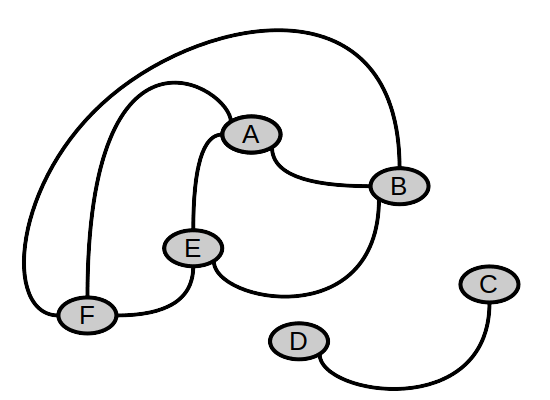
\includegraphics[width=0.4\textwidth]{structuresEx1.png}
\end{center}
&
6.\\
\hline
\item How many edges are there?
&
7.\\
\hline
\item What's the degree of vertex \textsl{B}?
&
3.\\
\hline
\item Is this graph directed?
&
No. (No arrowheads on the lines.)\\
\hline
\item Is this graph connected?
&
No -- there is no path from \textsl{A}, \textsl{B}, \textsl{E}, or \textsl{F}
to either \textsl{C} or \textsl{D}.\\
\hline
\item Is this graph weighted?
&
No. (No numbers annotating the edges.)\\
\hline
\item Is it a tree?
&
No. (A tree must be connected, and must also have no cycles, which this graph
clearly does: \textit{e.g.},
\textsl{B}--to--\textsl{A}--to--\textsl{E}--to--\textsl{B}.)\\
\hline
\item Is it a DAG?
&
Not remotely: it is neither directed nor acyclic.\\
\hline
\item If this graph represented an endorelation, how many ordered pairs would
it have?
&
14. (If you said 7, remember that since there are no arrowheads on the lines,
this is an undirected graph, which corresponds to a symmetric relation, and
hence both (\textsl{A}, \textsl{E}) and (\textsl{E}, \textsl{A}) will be
present.)\\


\hline
\vspace{-.2in}
\item How many vertices and edges are there in the graph below?
\begin{center}
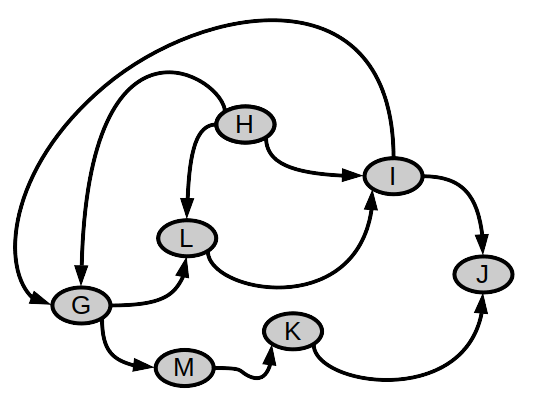
\includegraphics[width=0.4\textwidth]{structuresEx2.png}
\end{center}
&
7 and 10, respectively.\\
\hline
\vspace{-.2in}
\item What's the degree of vertex \textsl{L}?
&
\footnotesize
It has an in-degree of 2, and an out-degree of 1.\\
\hline
\normalsize
\vspace{-.2in}
\item Is this graph directed?
&
\footnotesize
Yes.\\
\hline
\normalsize
\item Is this graph connected?
&
\scriptsize
Depends on what we mean. There are two different notions of ``connectedness''
for directed graphs. One is \textbf{strongly connected}, which means every
vertex is reachable from any other by following the arrows in their specified
directions. By that definition, this graph is not connected: there's no way to
get to \textsl{H} from \textsl{J}, for example. It is \textbf{weakly
connected}, however, which means that if you \textit{ignore} the arrowheads and
consider it like an unidirected graph, it would be connected.\\
\hline
\normalsize
\item Is it a tree?
&
\scriptsize
No. For one thing, a tree can't have any ``extra'' edges beyond what's
necessary to make it connected, and there's redundancy galore here.\\
\hline
\normalsize
\item Is it a DAG?
&
\scriptsize
Allllmost. If you look very carefully, you'll see that there is indeed a cycle:
\textsl{I}--to--\textsl{G}--to--\textsl{L}. So if this graph were to represent
a recipe or project workflow, it would be impossible to complete.\\
\hline
\normalsize
\vspace{-.2in}
\item If we reversed the direction of the \textsl{I}--to--\textsl{G} edge,
would it be a DAG?
&
\footnotesize
Yes. The steps could now be completed in this order: \textsl{H}, \textsl{G},
\textsl{L}, \textsl{I}, \textsl{M}, \textsl{K}, and finally \textsl{J}.\\
\hline
\normalsize
\vspace{-.2in}
\item If this graph represented an endorelation, how many ordered pairs would
it have?
&
\footnotesize
10.\\
\hline
\vspace{-.2in}
\item Suppose we traversed the graph below in depth-first fashion, starting
with node \textsl{P}. In what order would we visit the nodes?
\begin{center}
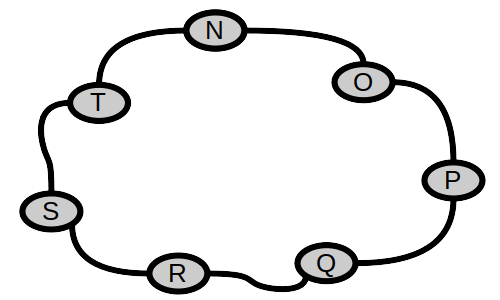
\includegraphics[width=0.4\textwidth]{structuresEx3.png}
\end{center}
&
There are two possible answers: \textsl{P}, \textsl{Q}, \textsl{R}, \textsl{S}, \textsl{T}, \textsl{N}, \textsl{O}, or else \textsl{P}, \textsl{O}, \textsl{N}, \textsl{T}, \textsl{S}, \textsl{R},
\textsl{Q}. (The choice just depends on whether we go ``left'' or ``right''
initially.) Note in particular that either \textsl{O} or \textsl{Q} is at the very end of the
list.\\
\hline
\vspace{-.2in}
\item Now we traverse the same graph breadth-first fashion, starting
with node \textsl{P}. Now in what order would we visit the nodes?
&
Again, two possible answers: \textsl{P}, \textsl{O}, \textsl{Q}, \textsl{N}, \textsl{R}, \textsl{T}, \textsl{S}, or else \textsl{P}, \textsl{Q}, \textsl{O}, \textsl{R}, \textsl{N}, \textsl{S},
\textsl{T}. Note in particular that both \textsl{O} and \textsl{Q} are visited
very early.\\
\hline
\item If we traversed the tree below in pre-order fashion, in what order would
we visit the nodes?
\begin{center}
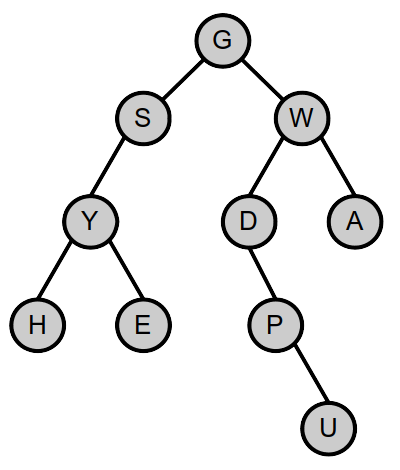
\includegraphics[width=0.4\textwidth]{structuresEx4.png}
\end{center}
&
\textsl{G}, \textsl{S}, \textsl{Y}, \textsl{H}, \textsl{E}, \textsl{W},
\textsl{D}, \textsl{P}, \textsl{U}, \textsl{A}.\\
\hline
\vspace{-.2in}
\item What if we traversed it in in-order fashion?
&
\textsl{H}, \textsl{Y}, \textsl{E}, \textsl{S}, \textsl{G}, \textsl{D},
\textsl{P}, \textsl{U}, \textsl{W}, \textsl{A}.\\
\hline
\vspace{-.2in}
\item What if we traversed it in post-order fashion?
&
\textsl{H}, \textsl{E}, \textsl{Y},\ \ \textsl{S}, \textsl{U}, \textsl{P},
\ \textsl{D}, \textsl{A}, \textsl{W}, \textsl{G}.\\
\hline
\item Is the graph below a tree?
\begin{center}
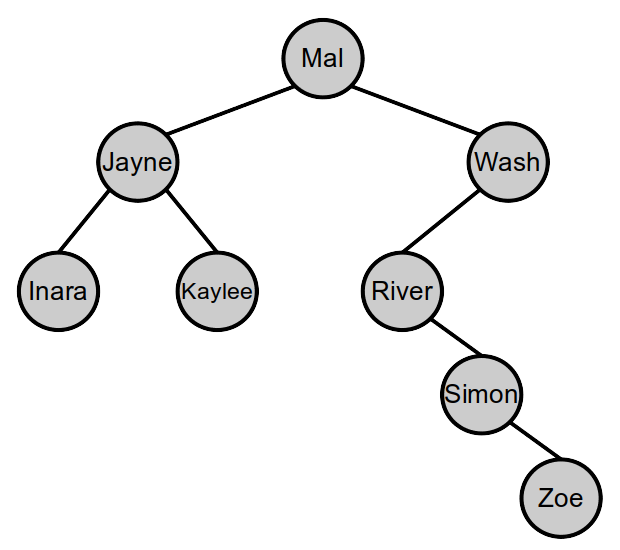
\includegraphics[width=0.4\textwidth]{structuresEx5.png}
\end{center}
&
Yes. (Every node has one and only one path to the root, and to every other node
for that matter.)\\
\hline
\item Is it a binary tree?
&
Yes. (Every node has at most two children, and they are clearly pictured as
being a ``left'' child and/or a ``right'' child.)\\
\hline
\item Is it a binary search tree?
&
No. Although nearly every node does satisfy the BST property (all the nodes in
its left subtree come before it alphabetically, and all the nodes in its right
subtree come after it), there is a single exception: \textsl{Zoe} is in
\textsl{Wash}'s left subtree, whereas she should be to his right.\\
\hline
\item How could we fix it?
&
Many ways; one would be to swap \textsl{Zoe}'s and \textsl{Wash}'s positions.\\
\hline
\item Is the tree balanced?
&
It's not too bad, but it does have one too many levels in it (it has a height
of 4, whereas all its nodes would fit in a tree of height 3).\\
\hline
\item How could we make it more balanced?
&
Many ways; one would be to make \textsl{Zoe} be \textsl{Wash}'s right child,
instead of \textsl{Simon}'s. \textsl{Simon} would then be a leaf. (Whether
\textsl{Zoe} would feel comfortable with this is another matter: \textsl{Zoe}'s
pretty alpha...)\\
\hline
\item If we wanted to add a new node called ``\textsl{Shepherd}'' to this tree,
where would he go?
&
To \textsl{Simon}'s left.\\
\hline
\item If we wanted to remove the ``\textsl{Mal}'' node from this tree, how
would we do that?
&
Two options include: put the right-most node of \textsl{Mal}'s left subtree
(that would be \textsl{Kaylee}) in \textsl{Mal}'s place, or put the left-most
node of \textsl{Mal}'s right subtree (that would be \textsl{River}) in
\textsl{Mal}'s place. In the former case, \textsl{Jayne} would simply lose his
right subchild; in the latter, \textsl{Simon} (and everything under him) would
become \textsl{Wash}'s left child.\\
\hline
\end{longtable}
\end{enumerate}
\end{small}
